\documentclass{assignment}
\UsingEnglish
\ProjectInfos*{Intro to Communication System}{EE140}{Fall, 2020}{Assignment 10}{Due time : 10:15, Dec 18, 2020 (Friday)}{陈稼霖}{45875852}
\begin{document}
\begin{prob}[5.12, Orthogonal subspace]
    For any subspace $\mathcal{S}$ of an inner product space $\mathcal{V}$, define $\mathcal{S}^{\perp}$ as the set of vectors $\bm{v}\in\mathcal{V}$ that are orthogonal to all $\bm{w}\in\mathcal{S}$.
    \begin{itemize}
        \item[(a)] Show that $\mathcal{S}^{\perp}$ is a subspace of $\mathcal{V}$.
        \item[(b)] Assuming that $\mathcal{S}$ is finite-dimensional, show that any $\bm{u}\in\mathcal{V}$ can be uniquely decomposed into $\bm{u}=\bm{u}_{\vert\mathcal{S}}+\bm{u}_{\perp\mathcal{S}}$, where $\bm{u}_{\vert\mathcal{S}}\in\mathcal{S}$ and $\bm{u}_{\perp\mathcal{S}}\in\mathcal{S}^{\perp}$.
        \item[(c)] Assuming that $\mathcal{V}$ is finite-dimensional, show that $\mathcal{V}$ has an orthonormal basis where some of the basis vectors form a basis for $\mathcal{S}$ and the remaining basis vectors form a basis for $\mathcal{S}^{\perp}$.
    \end{itemize}
\end{prob}
\begin{sol}
    \begin{itemize}
        \item[(a)] $\mathcal{S}^{\perp}$ satisfies the following two conditions:
        \begin{itemize}
            \item[(i)] $\bm{0}\in\mathcal{S}^{\perp}$, since $\bm{0}\in\mathcal{V}$ and $\bm{0}\cdot\bm{w}=0\;\forall\bm{w}=\mathcal{S}$;
            \item[(ii)] If $\bm{v}_1,\bm{v}_2\in\mathcal{S}^{\perp}$, i.e. $\bm{v}_1,\bm{v}_2\in\mathcal{V}$ and $\bm{v}_1\cdot\bm{w}=0$, $\bm{v}_2\cdot\bm{w}=0\;\forall\bm{w}\in\mathcal{S}$, then $\alpha\bm{v}_1+\beta\bm{v}_2\in\mathcal{V}$ and $(\alpha\bm{v}_1+\beta\bm{v}_2)\cdot\bm{w}=\alpha\bm{v}_1\cdot\bm{w}+\beta\bm{v}_2\cdot\bm{w}=0\;\forall\bm{w}\in\mathcal{S}$, so $\alpha\bm{v}_1+\beta\bm{v}_2\in\mathcal{S}^{\perp}$, where $\alpha,\beta$ are arbitrary scalars.
        \end{itemize}
        Therefore, $\mathcal{S}^{\perp}$ is a subspace of $\mathcal{V}$.
        \item[(b)] According to Projection theorem (Theorem 5.3.1), since $\mathcal{S}$ is a subspace of the inner product space $\mathcal{V}$, for any $\bm{u}\in\bm{V}$, there is a unique vector $\bm{u}_{\vert\mathcal{S}}\in\mathcal{S}$ such that $(\bm{u}-\bm{u}_{\vert\mathcal{S}})\cdot\bm{s}=0\;\forall\bm{s}\in\mathcal{S}$ where $\bm{u}-\bm{u}_{\vert\mathcal{S}}=\bm{u}_{\perp\mathcal{S}}\in\mathcal{S}^{\perp}$. Therefore, any $\rm{u}\in\mathcal{V}$ an be uniquely decomposed into $\bm{u}=\bm{u}_{\vert\mathcal{S}}+\bm{u}_{\perp\mathcal{S}}$, where $\bm{u}_{\vert\mathcal{S}}=\mathcal{S}$ and $\bm{u}_{\perp\mathcal{S}}\in\mathcal{S}^{\perp}$.
        \item[(c)] Since $\mathcal{S}$ is a subspace, we can find an orthonormal basis of $\mathcal{S}$, say, $\{\bm{s}_k\vert k=1,2,\cdots,n_1\}$. For any $\bm{u}_{\vert\mathcal{S}}\in\mathcal{S}$, we can decompose it uniquely into the linear combination of $\{\bm{s}_k\vert k=1,2,\cdots,n_1\}$: $\bm{u}_{\vert\mathcal{S}}=\sum_{k=1}^{n_1}\alpha_j\bm{s}_j$.\\
        Similarly, since $\mathcal{S}^{\perp}$ is a subspace, we can find an orthonormal basis of $\mathcal{S}^{\perp}$, say, $\{\bm{t}_j\vert j=1,2,\cdots,n_2\}$. For any $\bm{u}_{\perp\mathcal{S}}\in\mathcal{S}$, we can decompose it uniquely into the linear combination of $\{\bm{t}_j\vert j=1,2,\cdots,n_2\}$: $\bm{u}_{\perp\mathcal{S}}=\sum_{j=1}^{n_2}\beta_j\bm{t}_j$.\\
        Now we prove that $\{\bm{s}_k\vert k=1,2,\cdots,n_1\}\cup\{\bm{t}_j\vert j=1,2,\cdots,n_2\}$ is a orthonormal basis of $\mathcal{V}$:
        \begin{itemize}
            \item[(i)] $\{\bm{s}_k\vert k=1,2,\cdots,n_1\}\cup\{\bm{t}_j\vert j=1,2,\cdots,n_2\}$ is a basis of $\mathcal{S}$, since for any $\bm{u}\in\mathcal{V}$, we can first decompose it uniquely into $\bm{u}=\bm{u}_{\vert\mathcal{S}}+\bm{u}_{\perp\mathcal{S}}$, where $\bm{u}_{\vert\mathcal{S}}\in\mathcal{S}$ and $\bm{u}_{\perp\mathcal{S}}\in\mathcal{S}^{\perp}$, and then decompose it uniquely into $\bm{u}=\sum_{k=1}^{n_1}\alpha_k\bm{s}_k+\sum_{j=1}^{n_2}\beta_j\bm{t}_j$;
            \item[(ii)] $\{\bm{s}_k\vert k=1,2,\cdots,n_1\}\cup\{\bm{t}_j\vert j=1,2,\cdots,n_2\}$ is orthonormal, since $\{\bm{s}_k\vert k=1,2,\cdots,n_1\}$ is orthonormal, $\{\bm{t}_j\vert j=1,2,\cdots,n_2\}$ is orthonormal, and for any $\bm{s}_k$ and $\bm{t}_j$, the definition of $\mathcal{S}^{\perp}$ requires that $\bm{s}_k\cdot\bm{t}_j=0$.
        \end{itemize}
        Therefore, $\mathcal{V}$ has an orthonormal basis where some of the basis vectors form a basis for $\mathcal{S}$ and the remaining basis vectors form a basis for $\mathcal{S}^{\perp}$.
    \end{itemize}
\end{sol}

\begin{prob}[5.13, Othonormal expansion]
    Expand the function $\sinc(3t/2)$ as an orthonormal expansion in the set of functions $\{\sinc(t-n);-\infty<n<\infty\}$.
\end{prob}
\begin{sol}
\end{sol}

\begin{prob}[6.3]
    \begin{itemize}
        \item[(a)] Assume that the received signal in a $4$-PAM system is $V_k=U_k+Z_k$, where $U_k$ is the transmitted $4$-PAM signal at time $k$. Let $Z_k$ be independent of $U_k$ and Gaussian with density $f_Z(z)=\sqrt{1/2\pi}\exp(-z^2/2)$. Assume that the receiver chooses the signal $\tilde{U}_k$ closest to $V_k$. (It is shown in Chapter 8 that this detection rule minimizes $P_e$ for equiprobable signals.) Find the probability $P_e$ (in terms of Gaussian intervals) that $U_k\neq\tilde{U}_k$.
        \item[(b)] Evaluate the partial derivative of $P_e$ with respect to the third signal point $a_3$ (i.e. the positive inner signal point) at the point where $a_3$ is equal to its value $d/2$ in standard $4$-PAM and all other signal points are kept at $4$-PAM values. [Hint. This does not require any calculation.]
    \end{itemize}
\end{prob}
\begin{sol}
    \begin{itemize}
        \item[(a)] 
        \item[(b)] 
    \end{itemize}
\end{sol}

\begin{prob}[6.4, Nyquist]
    Suppose that the PAM modulated baseband waveform $u(t)=\sum_{k=-\infty}^{\infty}u_kp(t-kT)$ is received. That is, $u(t)$ is known, $T$ is known, and $p(t)$ is known. We want to determine the signals $\{u_k\}$ from $u(t)$. Assume only linear operations can be used. That is, we wish to find some waveform $d_k(t)$ for each integer $k$ such that $\int_{-\infty}^{\infty}u(t)d_k(t)\,\mathrm{d}t=u_k$.
    \begin{itemize}
        \item[(a)] What properties must be satisfied by $d_k(t)$ such that the above equation is satisfied no matter what values are taken by the other signals. $\cdots,u_{k-2},u_{k-1},u_{k+1},u_{k+2},\cdots$? These properties should take the from of constrains on the inner products $\langle p(t-kT),d_j(t)\rangle$. Do not worry about convergence, interchange of limits, etc.
        \item[(b)] Suppose you find a function $d_0(t)$ that satisfies these constrains for $k=0$. Shown that, for each $k$, a function $d_k(t)$ satisfying these constrains can be found simply in terms of $d_0(t)$.
        \item[(c)] What is the relationship between $d_0(t)$ and a function $q(t)$ that avoids intersymbol interference in the approach taken in Section 6.3 (i.e. a function $q(t)$ such that $p(t)*q(t)$ is ideal Nyquist)?
    \end{itemize}
    You have shown that the filter/sample approach in Section 6.3 is no less general than the arbitrary linear operation approach here. Note that, in the absence of noise and with a known constellation, it must be possible to retrieve the signals from the waveform using nonlinear operations even in the presence of intersymbol interference.
\end{prob}
\begin{sol}
    \begin{itemize}
        \item[(a)] 
        \item[(b)] 
        \item[(c)] 
    \end{itemize}
\end{sol}

\begin{prob}[6.5, Nyquist]
    Let $v(t)$ be a continuous $\mathcal{L}_2$ waveform with $v(0)=1$ and define $g(t)=v(t)\sinc(t/T)$.
    \begin{itemize}
        \item[(a)] Show that $g(t)$ is ideal Nyquist with interval $T$.
        \item[(b)] Find $\hat{g}(f)$ as a function of $\hat{v}(f)$.
        \item[(c)] Give a direct demonstration that $\hat{g}(f)$ satisfies the Nyquist criterion.
        \item[(d)] If $v(t)$ is baseband-limited to $B_b$, what is $g(t)$ baseband-limited to?
    \end{itemize}
\end{prob}
\begin{sol}
    \begin{itemize}
        \item[(a)] 
        \item[(b)] 
        \item[(c)] 
        \item[(d)] 
    \end{itemize}
\end{sol}

\begin{prob}[6.6, Nyquist]
    Consider a PAM baseband system in which the modulator is defined by a signal interval $T$ and a waveform $p(t)$, the channel is defined by a filter $h(t)$, and the receiver is defined by a a filter $q(t)$ which is sampled at $T$-spaced intervals. The received waveform, after the receiver filter $q(t)$, is then given by $r(t)=\sum_ku_kg(t-kT)$, where $g(t)=p(t)*h(t)*q(t)$.
    \begin{itemize}
        \item[(a)] What properties must $g(t)$ have so that $r(kT)=u_k$ for all $k$ and for all choices of input $\{u_k\}$? What is the Nyquist criterion for $\hat{g}(f)$?
        \item[(b)] Now assume that $T=1/2$ and that $p(t)$, $h(t)$, $q(t)$ and all their Fourier transforms are restricted to be real. Assume further that $\hat{p}(f)$ and $\hat{h}(f)$ are specified by \ref{Figure 6.10}, i.e. by
        \[
            \hat{p}(f)=\left\{\begin{array}{ll}
                1&\abs{f}\leq 0.5;\\
                1.5-t&0.5<\abs{f}\leq 1.5;\\
                0&\abs{f}>1.5;
            \end{array}\right.\qquad\hat{h}(f)=\left\{\begin{array}{ll}
                1&\abs{f}\leq 0.75;\\
                0&0.75<\abs{f}\leq 1;\\
                1&1<\abs{f}\leq 1.25;\\
                0&\abs{f}>1.25.
            \end{array}\right.
        \]
        \begin{figure}[h]
            \centering
            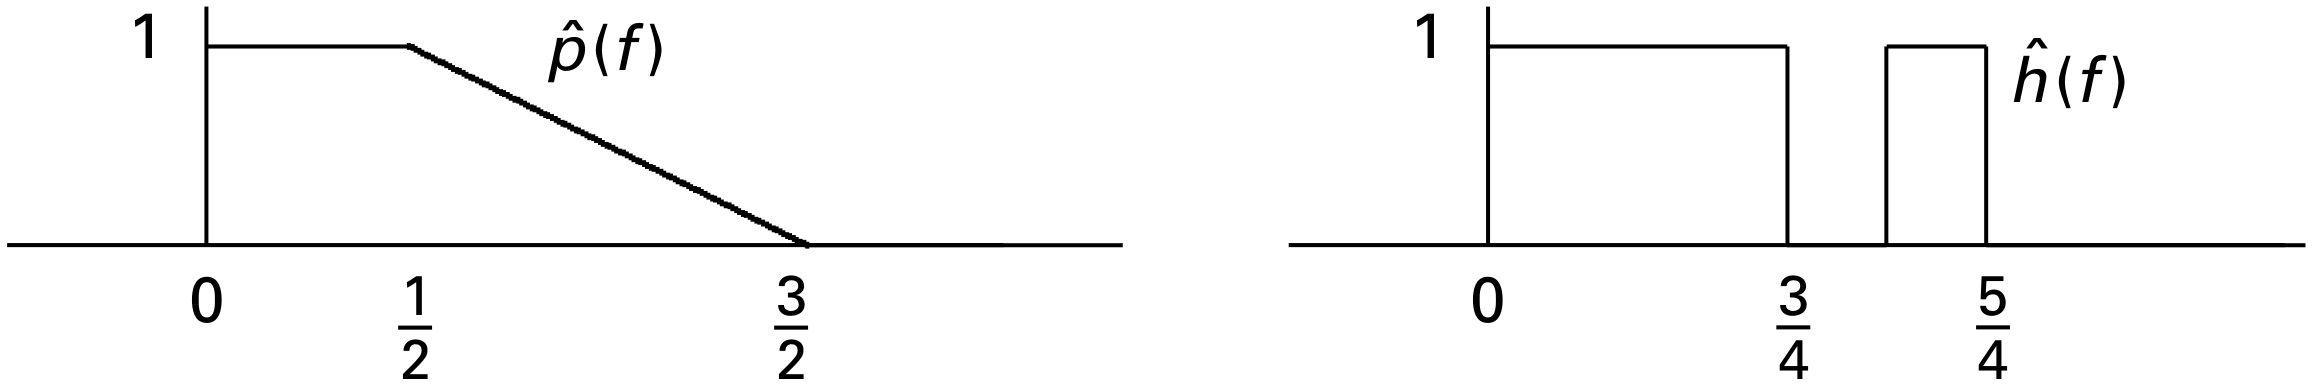
\includegraphics[width=.5\columnwidth]{Assignment-10-Figure-6.10.png}
            \caption{}
            \label{Figure 6.10}
        \end{figure}
        Is it possible to choose a receiver filter transform $\hat{q}(f)$ so that there is no intersymbol interference? If so, give such a $\hat{q}(f)$ and indicate the regions in which your solution is nonunique.
        \item[(c)] Redo part (b) with the modification that now $\hat{h}(f)=1$ for $\abs{f}\leq 0.75$ and $\hat{h}(f)=0$ for $\abs{f}>0.75$.
        \item[(d)] Explain the conditions on $\hat{p}(f)\hat{h}(f)$ under which intersymbol interference can be avoided by proper choice of $\hat{q}(f)$. (You may assume, as above, that $\hat{p}(f)$, $\hat{h}(f)$, $p(t)$, and $h(t)$ are all real.)
    \end{itemize}
\end{prob}
\begin{sol}
    \begin{itemize}
        \item[(a)] 
        \item[(b)] 
        \item[(c)] 
        \item[(d)] 
    \end{itemize}
\end{sol}

\begin{prob}[6.16, Passband expansion] Prove Theorem 6.6.1. [Hint. First show that the set of functions $\{\hat{\psi}_{k,1}(f)\}$ and $\{\hat{\psi}_{k,2}(f)\}$ are orthogonal with energy $2$ by comparing the integral over negative frequencies with that over positive frequencies.] Indicate explicitly why you need $f_c>B/2$.

    \begin{framed}
        \textbf{Theorem 6.6.1} \itshape Let $\{\theta_k(t):k\in\mathbb{Z}\}$ be an orthonormal set limited to the frequency band $[-B/2,B/2]$. Let $f_e$ be greater than $B/2$, and for each $k\in\mathbb{Z}$ let
        \begin{align*}
            \psi_{k,1}(t)=&\re[2\theta_k(t)e^{2\pi if_ct}],\\
            \psi_{k,2}(t)=&\im[-2\theta_k(t)e^{2\pi if_ct}].
        \end{align*}
        The set $\{\psi_{k,j};k\in\mathbb{Z},j\in\{1,2\}\}$ is an orthogonal set of functions, each with energy $2$. Furthermore if $u(f)=\sum_ku_k\theta_k(t)$, then the corresponding passband function $x(t)=2\re[u(t)e^{2\pi if_ct}]$ is given by
        \[
            x(t)=\sum_k\re[u_k]\psi_{k,1}(t)+\im[u_k]\psi_{k,2}(t).
        \]
    \end{framed}
\end{prob}
\begin{sol}
\end{sol}
\end{document}